\documentclass[conference]{IEEEtran}
\usepackage[T1]{fontenc}
\usepackage{graphicx,booktabs,amsmath,amssymb,siunitx,cite,url}
\usepackage[hidelinks]{hyperref}
\graphicspath{{../figures/}}
\sisetup{group-separator={,},group-minimum-digits=4}
% Generated by scripts/write_latex_numbers.py from reports/jc_pinn_20261107/. Do not edit by hand.
\newcommand{\nAdamLR}{0.005}
\newcommand{\nAdamSteps}{1{,}500}
\newcommand{\nAlpha}{1}
\newcommand{\nCasesHigh}{17}
\newcommand{\nCasesLow}{20}
\newcommand{\nColloc}{4{,}096}
\newcommand{\nCtrlCV}{1.315}
\newcommand{\nCtrlGroups}{5.629}
\newcommand{\nCtrlScore}{3.472}
\newcommand{\nCtrlTest}{0.338}
\newcommand{\nCtrlTestWorst}{0.612}
\newcommand{\nDeltaMax}{0.917}
\newcommand{\nDeltaMean}{0.466}
\newcommand{\nEnsGroups}{6.79}
\newcommand{\nEnsTest}{0.059}
\newcommand{\nEqA}{148.77}
\newcommand{\nEqB}{526.23}
\newcommand{\nEqC}{0.0292}
\newcommand{\nEqCV}{10.24}
\newcommand{\nEqGroups}{13.95}
\newcommand{\nEqm}{1.11}
\newcommand{\nEqn}{0.828}
\newcommand{\nEqq}{0.717}
\newcommand{\nEqr}{0}
\newcommand{\nFloorCubicMean}{0.30}
\newcommand{\nFloorJCMean}{0.84}
\newcommand{\nFloorJCMedian}{0.51}
\newcommand{\nImprovement}{17}
\newcommand{\nLbfgsIter}{2{,}500}
\newcommand{\nLookupCV}{3.60}
\newcommand{\nLookupGroups}{13.96}
\newcommand{\nMemberBest}{0.390}
\newcommand{\nMemberWorst}{0.478}
\newcommand{\nNumpyTorchErr}{3.4e-13}
\newcommand{\nParams}{385}
\newcommand{\nPinnA}{87.72}
\newcommand{\nPinnB}{424.64}
\newcommand{\nPinnC}{0.0518}
\newcommand{\nPinnm}{2.74}
\newcommand{\nPinnn}{0.942}
\newcommand{\nPinnq}{0.911}
\newcommand{\nPinnr}{2.1e-05}
\newcommand{\nRunMinutes}{37}
\newcommand{\nScrAlphaLow}{4.072}
\newcommand{\nScrBoundedScore}{9.24}
\newcommand{\nScrIterLong}{2.150}
\newcommand{\nScrWide}{2.878}
\newcommand{\nSelCV}{2.098}
\newcommand{\nSelCVMedian}{0.592}
\newcommand{\nSelCVWorst}{20.58}
\newcommand{\nSelGroups}{6.235}
\newcommand{\nSelScore}{4.166}
\newcommand{\nSettings}{14}
\newcommand{\nSingleCV}{2.17}
\newcommand{\nSingleGroups}{11.90}
\newcommand{\nSingleTest}{0.143}
\newcommand{\nSpreadMax}{0.338}
\newcommand{\nSpreadMean}{0.104}
\newcommand{\nTestBest}{0.093}
\newcommand{\nTestBestCase}{37}
\newcommand{\nTestBias}{+0.009}
\newcommand{\nTestCases}{37}
\newcommand{\nTestCasesSplit}{37}
\newcommand{\nTestEq}{7.37}
\newcommand{\nTestEqWorst}{13.47}
\newcommand{\nTestLookup}{1.379}
\newcommand{\nTestMAE}{0.327}
\newcommand{\nTestMaxAbs}{2.90}
\newcommand{\nTestMaxPct}{9.2}
\newcommand{\nTestMean}{0.439}
\newcommand{\nTestMeanPct}{0.38}
\newcommand{\nTestMedian}{0.395}
\newcommand{\nTestPoints}{4{,}440}
\newcommand{\nTestRsq}{0.99952}
\newcommand{\nTestWithinHalf}{80.2}
\newcommand{\nTestWithinOne}{94.9}
\newcommand{\nTestWithinTwo}{98.8}
\newcommand{\nTestWorst}{0.841}
\newcommand{\nTestWorstCase}{10}
\newcommand{\nTrainCases}{36}
\newcommand{\nTrainFit}{0.356}
\newcommand{\nWinsEnsemble}{0}
\newcommand{\nWinsEq}{37}
\newcommand{\nWinsLookup}{24}
\newcommand{\nWinsSingle}{0}

\newcommand{\sjc}{\sigma_{\mathrm{JC}}}

\begin{document}
\title{JC-PINN: A Customised Johnson--Cook Law as the Governing Equation of a Neural Material Model for Additively Manufactured AlSi10Mg}
\author{\IEEEauthorblockN{Team 8}\IEEEauthorblockA{Multiscale Modelling of Materials using Machine Learning, course project\\November 2026}}
\maketitle

\begin{abstract}
We embed a customised Johnson--Cook law as the backbone of a neural material model for the simulated von Mises stress of additively manufactured AlSi10Mg. The law covers strain, strain rate, temperature, shear modulus and porosity. The model multiplies the law by $\exp(\delta)$, where $\delta$ is a 5--16--16--1 tanh correction (\nParams{} weights) whose output layer starts at zero, so training begins from the law itself. Physics residuals at \nColloc{} collocation points, frozen against jointly fitted constants and five seeds were compared using training data only, with a score balancing case-wise cross-validation and held-out temperature/rate groups. The model was locked before testing. On \nTestCasesSplit{} test simulations the mean per-curve RMSE is \nTestMean{}~MPa ($R^2=\nTestRsq$, \nTestWithinOne\,\% of points within $\pm1$~MPa). This is \nImprovement{} times better than the law alone and roughly half the single-MLP error on unseen conditions. Data-driven MLPs remain more precise on the random split, and a control without the law was slightly better, so the law contributes structure and interpretability rather than accuracy. We report these results and their limits.
\end{abstract}

\begin{IEEEkeywords}
physics-informed machine learning, Johnson--Cook model, AlSi10Mg, additive manufacturing, porosity, constitutive modelling, neural network
\end{IEEEkeywords}

\section{Introduction}
Porosity in laser-powder-bed-fused AlSi10Mg changes density, stiffness and flow stress~\cite{kempen2012}. A multiscale analysis of an AM wing-rib bracket therefore needs a material response that is cheap to evaluate across temperature, rate and porosity.

Purely data-driven surrogates fit such simulations closely but encode no physics. Physics-informed learning instead adds known equations to training~\cite{raissi2019,karniadakis2021,willard2022}. For constitutive behaviour, physics has been built into networks through thermodynamics~\cite{masi2021} and recurrent state~\cite{mozaffar2019}. Physics losses can also make optimisation harder~\cite{krishnapriyan2021}.

We take a simpler route. Our governing equation is a customised Johnson--Cook (JC) law~\cite{johnson1983}, which serves as a multiplicative backbone. Our contributions:
\begin{enumerate}
\item a JC-PINN model that starts as the law and learns only a correction;
\item a leakage-controlled protocol, with selection on training data only and a lock before testing;
\item a candid evaluation that includes a control without the law and a screen for improvements.
\end{enumerate}

\section{Related work}
Physics-informed neural networks add the residual of a governing equation to the loss, evaluated at collocation points where no data exist~\cite{raissi2019}. The idea has spread from fluid and wave problems to materials and engineering systems~\cite{karniadakis2021,willard2022}.

For constitutive modelling, two lines are prominent:
\begin{itemize}
\item thermodynamics-based networks, which build free energy and dissipation into the architecture~\cite{masi2021};
\item recurrent networks, which learn path-dependent plasticity from many loading paths~\cite{mozaffar2019}.
\end{itemize}
Both need quantities, such as internal variables and thousands of paths, that our data do not provide. Physics losses can also be hard to balance against data losses~\cite{krishnapriyan2021}.

A third, lighter option keeps a closed-form law and learns a correction to it. Our work follows that option with the JC family~\cite{johnson1983}. Two choices distinguish it:
\begin{itemize}
\item the law is a multiplicative backbone and the network starts from it exactly;
\item the physics residual is treated as a hyper-parameter, chosen by held-out evidence, rather than assumed to help.
\end{itemize}

\section{Data}
The supplied set contains 73 of 108 planned simulations: 27 at 30\,\textdegree C, 27 at 100\,\textdegree C, 19 at 200\,\textdegree C and none at 300\,\textdegree C. The strain rate is $10^{-5}$--$10^{-3}$\,s$^{-1}$, the density 2488--2700\,kg\,m$^{-3}$ and the shear modulus $G$ 23314--25300\,MPa. Units are inferred.

The target is $S_{vm}$ along the axial strain $E_{11}$, resampled to 120 strains in $[0.0002,0.0999]$. Every curve softens, and the softening grows with temperature (Fig.~\ref{fig:data}). We use the project's fixed split by simulation (seed 42): \nTrainCases{} training and \nTestCasesSplit{} test cases. Earlier project stages explored the test cases, so the test is not blind.

\begin{figure}[t]\centering
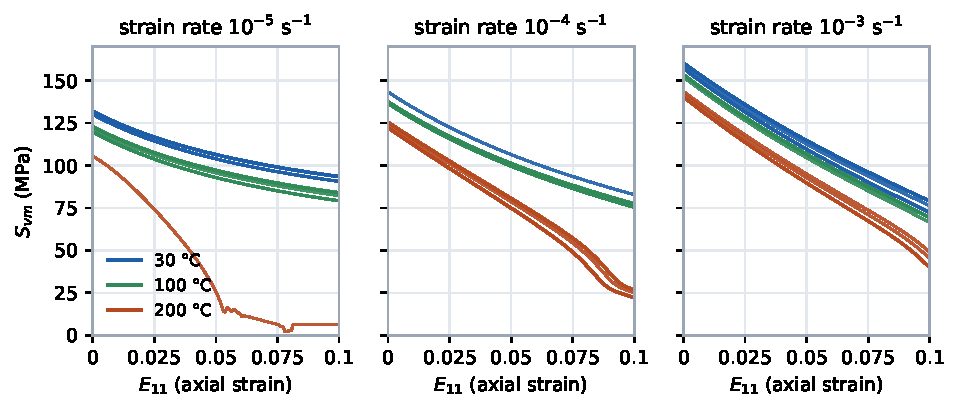
\includegraphics[width=\columnwidth]{fig_data}
\caption{Training curves by rate and temperature. All soften; the softening grows with temperature.}
\label{fig:data}
\end{figure}

\section{Governing equation}
The customised law (Equation~1) is
\begin{equation}
\sjc=[A-B\varepsilon^{n}][1+C\ln\dot\varepsilon^*][1-T^{*m}][G/G_0]^{q}[1-\phi]^{r},
\end{equation}
with
\begin{itemize}
\item $\varepsilon=E_{11}$ and $\dot\varepsilon^*=\dot\varepsilon/10^{-5}$;
\item $T^*=(T-30)/(600-30)$;
\item $G_0=25300$\,MPa;
\item $\phi=1-\rho/2700$.
\end{itemize}
The minus sign in the strain term reflects softening. The constants are bounded: $B=A\beta/0.1^n$ with $0\le\beta\le0.99$, which keeps the strain term positive, and $C,q,r\ge0$, which enforce the observed trend signs.

The law is separable, so the conditions can only rescale a curve, not reshape it. Fitted alone, it reaches a case-wise CV of \nEqCV{}~MPa and a test error of \nTestEq{}~MPa (Fig.~\ref{fig:eqfail}), with $A=\nEqA$, $B=\nEqB$, $n=\nEqn$, $C=\nEqC$, $m=\nEqm$, $q=\nEqq$ and $r=0$.

\begin{figure}[t]\centering
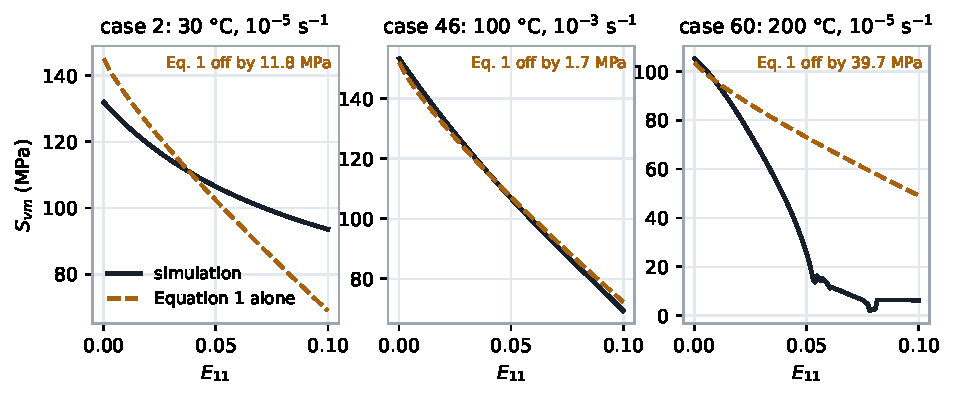
\includegraphics[width=\columnwidth]{fig_eq1_fail}
\caption{Equation~1 calibrated alone (dashed) cannot bend its curve differently at different conditions.}
\label{fig:eqfail}
\end{figure}

\section{Model and training}
The model is
\begin{equation}
\hat\sigma=\sjc(\mathbf x;\theta)\,\exp\bigl(\delta(\mathbf z)\bigr),\quad \mathbf z=(\mathbf x-\boldsymbol\mu)/\mathbf s,
\end{equation}
with inputs $\mathbf x=(T,\log_{10}\dot\varepsilon,\rho,G,E_{11})$. The correction $\delta$ is a 5--16--16--1 tanh network whose output layer starts at zero (Fig.~\ref{fig:arch}). Five copies (seeds 0--4) are combined by geometric mean.

The loss is
\begin{equation}
\mathcal L=\overline{((\hat\sigma-\sigma)/s_y)^2}+\lambda\,\overline{R^2}+\tfrac{\alpha}{N}\textstyle\sum W^2 ,
\end{equation}
with $\alpha=\nAlpha$. The residual $R$ is evaluated at \nColloc{} scrambled Sobol points~\cite{sobol1967} spanning the planned design box, 30--300\,\textdegree C. It takes one of two forms:
\begin{itemize}
\item \emph{level}: $R=\delta$;
\item \emph{trend}: $R=\partial\delta/\partial(T,\log\dot\varepsilon,\rho,G)$, computed by automatic differentiation.
\end{itemize}

Training runs in PyTorch~\cite{paszke2019}: \nAdamSteps{} Adam~\cite{kingma2014} steps at learning rate \nAdamLR, then up to \nLbfgsIter{} L-BFGS~\cite{liu1989} iterations. The constants are either frozen after a bounded least-squares calibration (SciPy~\cite{virtanen2020}) or trained jointly. Fig.~\ref{fig:train} shows one copy training: the prediction moves from the law's shape to the simulation's.

\begin{figure}[t]\centering
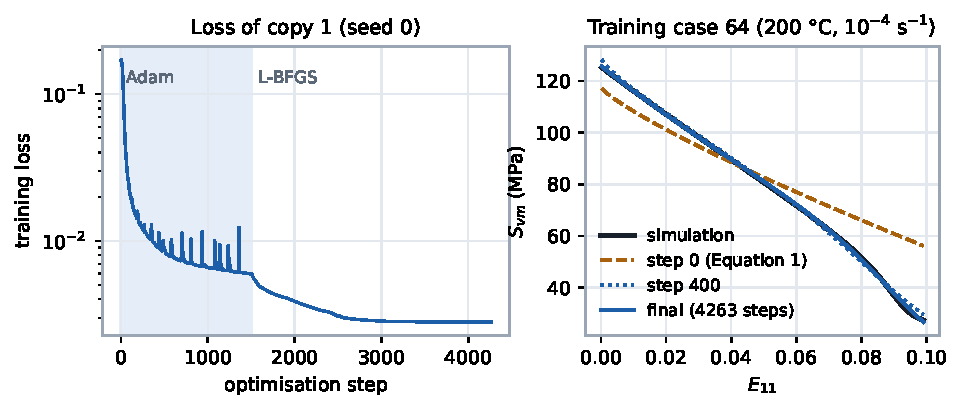
\includegraphics[width=\columnwidth]{fig_training}
\caption{Training of one copy: loss (left), and a 200\,\textdegree C training curve moving from Equation~1 (step 0) to the simulation (right).}
\label{fig:train}
\end{figure}

\begin{figure}[t]\centering
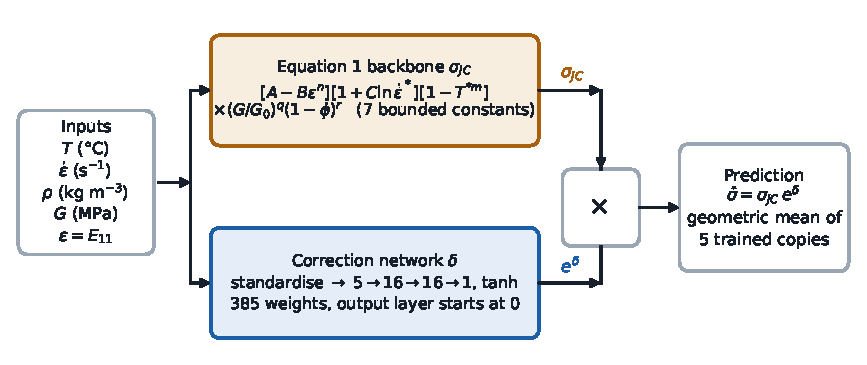
\includegraphics[width=\columnwidth]{fig_architecture}
\caption{The JC-PINN: Equation~1 times $\exp(\delta)$ from a zero-initialised correction network.}
\label{fig:arch}
\end{figure}

\section{Selection and lock}
We compared \nSettings{} settings on the training cases only, each with three seeds:
\begin{itemize}
\item no physics loss;
\item the level residual with $\lambda\in\{10^{-3},10^{-2},10^{-1}\}$;
\item the trend residual with $\lambda\in\{10^{-4},10^{-3},10^{-2}\}$;
\end{itemize}
and each of these with frozen or joint constants.

The score is $\tfrac12$(three-fold case CV $+$ the mean RMSE over nine held-out temperature/rate groups). The best was \emph{no physics loss, joint constants}: CV \nSelCV, groups \nSelGroups, score \nSelScore. Every stronger physics weight scored worse (Table~\ref{tab:sel}, Fig.~\ref{fig:sel}).

\begin{figure*}[t]\centering
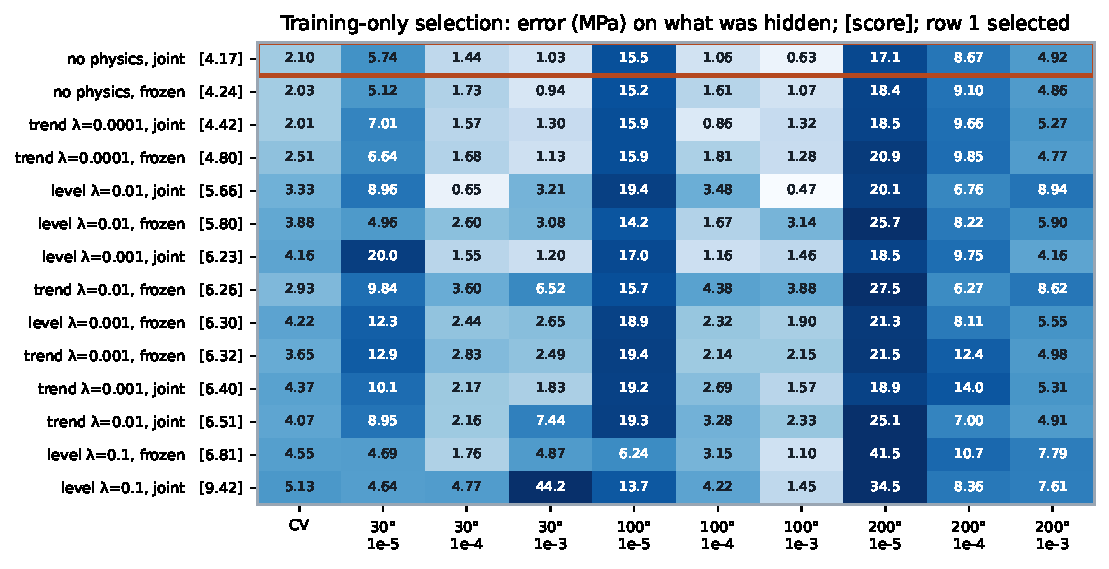
\includegraphics[width=.86\textwidth]{fig_selection}
\caption{Training-only selection of the \nSettings{} settings: case-CV error and the error on each hidden group (MPa), with the score in brackets. Row~1 was selected.}
\label{fig:sel}
\end{figure*}

The final model was fingerprinted (SHA-256) and saved before any test curve was read. The jointly fitted constants are $A=\nPinnA$, $B=\nPinnB$, $n=\nPinnn$, $C=\nPinnC$, $m=\nPinnm$, $q=\nPinnq$ and $r\approx0$.

\begin{table}[t]\centering\small
\caption{Training-only selection (MPa). Lower is better.}
\label{tab:sel}
\begin{tabular}{lrrr}\toprule
Setting & CV & Groups & Score\\\midrule
\textbf{none, joint (selected)} & \textbf{\nSelCV} & \textbf{\nSelGroups} & \textbf{\nSelScore}\\
none, frozen & 2.032 & 6.441 & 4.237\\
trend $10^{-4}$, joint & 2.010 & 6.822 & 4.416\\
trend $10^{-4}$, frozen & 2.505 & 7.101 & 4.803\\
level $10^{-2}$, joint & 3.332 & 7.997 & 5.664\\
level $10^{-1}$, joint & 5.130 & 13.714 & 9.422\\\midrule
Equation 1 alone & \nEqCV & \nEqGroups & --\\\bottomrule
\end{tabular}
\end{table}

\section{Results}
\subsection{Test accuracy and precision}
Scored once on \nTestCasesSplit{} cases (\nTestPoints{} points), the mean curve RMSE is \nTestMean{}~MPa (median \nTestMedian, worst \nTestWorst{} at case~\nTestWorstCase). Further:
\begin{itemize}
\item $R^2=\nTestRsq$;
\item \nTestWithinHalf\,\% of points are within $\pm0.5$~MPa and \nTestWithinOne\,\% within $\pm1$~MPa (Fig.~\ref{fig:pts});
\item the bias is \nTestBias~MPa, with \nCasesHigh{} cases above and \nCasesLow{} below;
\item the five copies differ by \nSpreadMean~MPa on average;
\item the training fit (\nTrainFit) is close to the test error, so there is no sign of over-fitting.
\end{itemize}
The worst eight cases share one condition (30\,\textdegree C, $10^{-4}$\,s$^{-1}$), which has a single training case. Fig.~\ref{fig:ex} shows the best, median and worst cases.

\begin{figure}[t]\centering
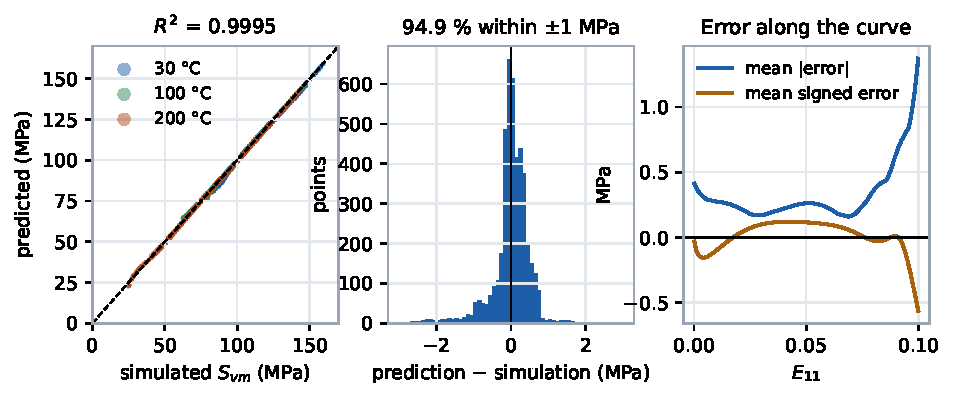
\includegraphics[width=\columnwidth]{fig_test_points}
\caption{Test points: parity, error histogram, and error along the strain axis.}
\label{fig:pts}
\end{figure}

\begin{figure*}[t]\centering
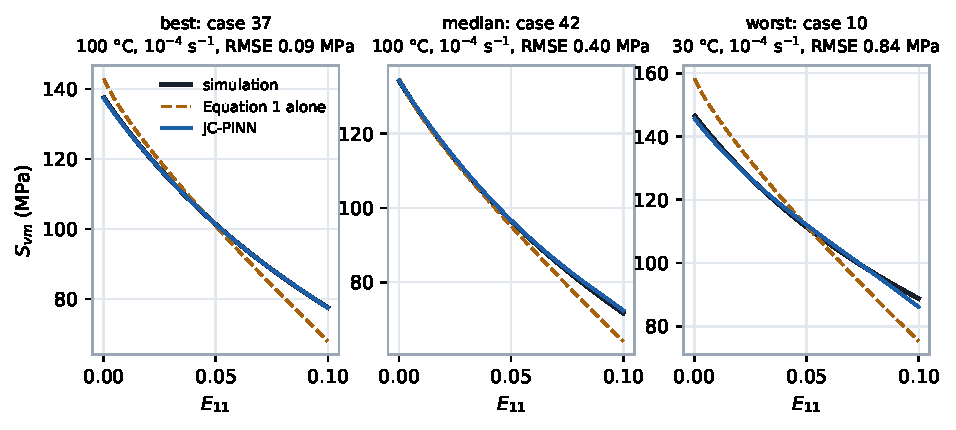
\includegraphics[width=.8\textwidth]{fig_test_examples}
\caption{Best, median and worst test cases: simulation, Equation~1 alone and the JC-PINN.}
\label{fig:ex}
\end{figure*}

\subsection{Comparison and control}
Table~\ref{tab:cmp} compares models on the same split. The JC-PINN:
\begin{itemize}
\item beats the law alone on all \nWinsEq{} test cases and a nearest-curve lookup on \nWinsLookup;
\item beats neither earlier MLP on any case;
\item on unseen groups, has about half the single-MLP error (Fig.~\ref{fig:groups}). This figure is somewhat optimistic, because the groups entered selection.
\end{itemize}
A post-hoc control, the same network with the law replaced by a constant and not used for selection, was better on every measure. On these data, therefore, the separable law adds interpretability (named constants, correct trends, a sensible starting point) but not accuracy.

\begin{table}[t]\centering\small
\caption{Mean curve RMSE (MPa) on the same 36/37 split.}
\label{tab:cmp}
\begin{tabular}{lrrr}\toprule
Model & Case CV & Groups & Test\\\midrule
Equation 1 alone & \nEqCV & \nEqGroups & \nTestEq\\
Nearest-curve lookup & \nLookupCV & \nLookupGroups & \nTestLookup\\
\textbf{JC-PINN} & \textbf{\nSelCV} & \textbf{\nSelGroups} & \textbf{\nTestMean}\\
Control (law off) & \nCtrlCV & \nCtrlGroups & \nCtrlTest\\
Single MLP & \nSingleCV & \nSingleGroups & \nSingleTest\\
Five-MLP ensemble & -- & \nEnsGroups$^{\ast}$ & \nEnsTest\\\bottomrule
\multicolumn{4}{l}{\footnotesize $^{\ast}$Different holdout folds.}
\end{tabular}
\end{table}

\begin{figure}[t]\centering
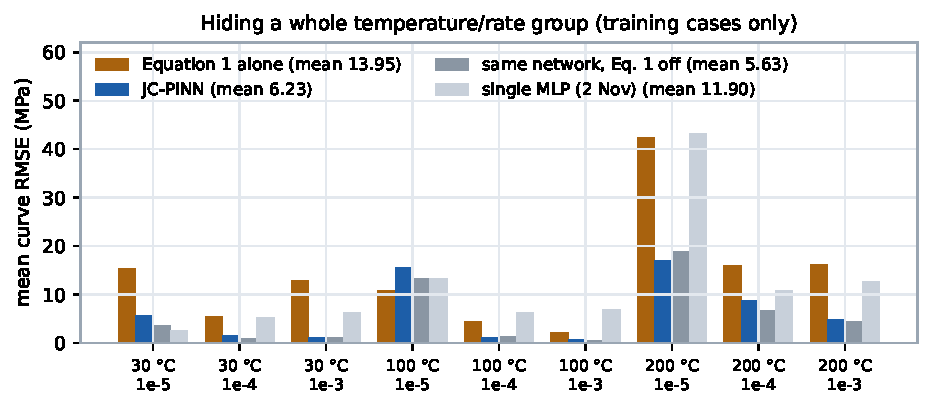
\includegraphics[width=\columnwidth]{fig_groups}
\caption{Error when a whole temperature/rate group is hidden (training cases only).}
\label{fig:groups}
\end{figure}

\begin{figure}[t]\centering
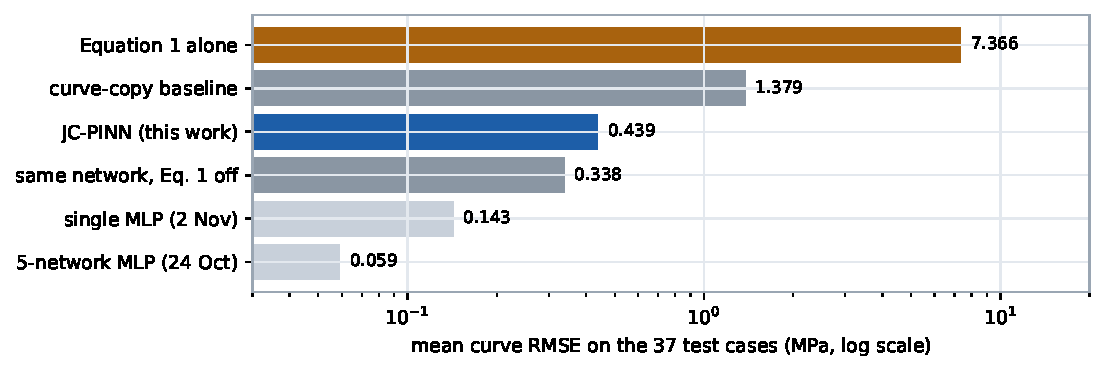
\includegraphics[width=\columnwidth]{fig_comparison}
\caption{Mean curve RMSE on the 37 test cases (log scale).}
\label{fig:cmp}
\end{figure}

\subsection{Physical behaviour}
Across 2579 points in the observed range (30--200\,\textdegree C), the predicted stress falls with strain and with temperature, and rises with $G$ and with density, at every point. Fig.~\ref{fig:study} shows curves at the project's study porosity $\phi=4\,\%$. The 300\,\textdegree C curves are unvalidated extrapolation: no data exist there, and no physics penalty is active.

\textbf{Porosity.} Porosity enters only through density ($\phi=1-\rho/2700$). In all \nPorPairsLower{} of \nPorPairs{} case pairs that differ in density alone, lower density gives lower stress. Over $\phi=0\to7.85\,\%$ the drop is \nPorData\,\% (\nPorDataThirty, \nPorDataHundred{} and \nPorDataTwoHundred\,\% at 30, 100 and 200\,\textdegree C). That is about \nPorRatio{} times weaker than the effect of $G$.

The data imply $r\approx\nPorImpliedR$, but the separable fit sets $r=0$: the effect is buried under Equation~1's misfit. The correction network instead reproduces it, through the density input: \nPorModel\,\% against \nPorData\,\%, the same sign in every pair, and correlation \nPorFullCorr{} (Fig.~\ref{fig:por}). For a real part, the effect of porosity therefore depends mainly on the unknown relation $G(\phi)$.

\begin{figure}[t]\centering
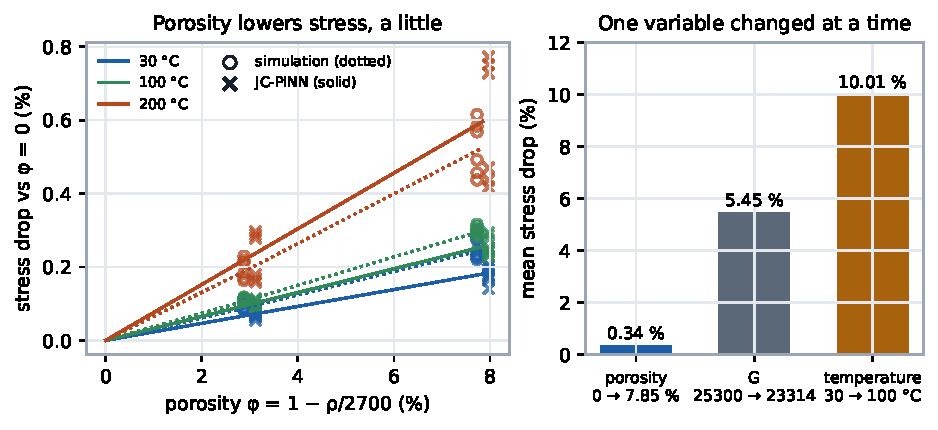
\includegraphics[width=\columnwidth]{fig_porosity}
\caption{Porosity effect: pairs differing only in density, simulation against JC-PINN (left), and one-variable effects (right).}
\label{fig:por}
\end{figure}

\begin{figure}[t]\centering
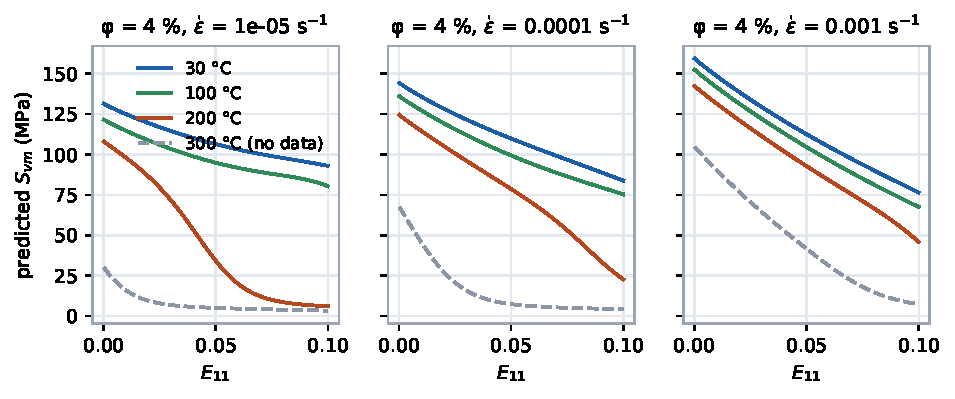
\includegraphics[width=\columnwidth]{fig_study_point}
\caption{Predicted curves at $\phi=4\,\%$ ($\rho=2592$, $G=24541$). Dashed: 300\,\textdegree C, no data.}
\label{fig:study}
\end{figure}

\subsection{Improvement screen}
After the lock, alternatives were screened on the training cases only:
\begin{itemize}
\item \textbf{Longer training} (CV \nScrIterLong), weaker weight decay (\nScrAlphaLow) and a wider network (\nScrWide) were all worse than \nSelCV.
\item \textbf{Per-curve strain law.} Fitting $A-B\varepsilon^n$ to each curve separately leaves \nFloorJCMean~MPa (a cubic reaches \nFloorCubicMean), so the power law is itself a floor, and a correction is required.
\item \textbf{Bounded or additive corrections} scored worse (for example \nScrBoundedScore{} against \nSelScore).
\end{itemize}
The locked model is kept.

\section{Discussion}
\textbf{Why did the physics residual not help?} The level residual pulls the model towards a law that is \nImprovement{} times less accurate than the data allow, so it trades accuracy for nothing in the observed range. The trend residual is gentler: at the smallest weight it was nearly tied with the selected setting. But the group holdouts show no gain at unseen conditions.

\textbf{What does the law buy?} The law's main contributions on these data are:
\begin{itemize}
\item a sensible starting point;
\item named constants for strain, rate, temperature, modulus and porosity;
\item a backbone that extrapolates in a physically shaped way.
\end{itemize}
These have value for explanation and for review, but the control shows they did not improve accuracy.

\textbf{What would change the picture?} Data at 300\,\textdegree C would test extrapolation directly, and a residual tied to measured trends could then be judged on evidence. A strain law that can change shape with condition would also help, because the per-curve floor shows the power law is the binding limit.

\section{Reproducibility and limits}
\textbf{Reproducibility.} An independent NumPy~\cite{harris2020} verifier reproduces every prediction to \nNumpyTorchErr~MPa. A Colab/Kaggle notebook retrains the model and reproduces the locked weights exactly. All quoted numbers are generated from the saved run.

\textbf{Limits.}
\begin{itemize}
\item The test is not blind.
\item The data are simulations, not experiments, and the units are inferred.
\item No data, and in the selected model no physics penalty, constrain predictions above 200\,\textdegree C.
\item The strain is total, not plastic.
\item The porosity--modulus relation of a real part is not defined by the data.
\item Fracture (critical flaw length) is not predicted.
\end{itemize}

\section{Conclusion}
A customised JC law works as the governing backbone of a neural material model. The model is \nImprovement{} times more accurate than the law alone and clearly better than a plain MLP on unseen conditions. It keeps physically named constants. Physics residuals did not help here, and a law-free control matched or beat it. The next steps are data at 300\,\textdegree C, experimental validation and a measured porosity--modulus relation.

\bibliographystyle{IEEEtran}
\bibliography{../report/refs}
\end{document}
